\documentclass[12pt]{article}

%%% CW says:
%%%
%%%\documentclass[12pt]{article}
%%%\usepackage{hyperref}
%%% this throws an error:
%%%
%%% (/usr/local/texlive/2011/texmf-dist/doc/latex/listings-ext/hyperref.cfg
%%% 
%%% ! Package hyperref Error: Wrong DVI mode driver option `ps2pdf',
%%% (hyperref)                because pdfTeX or LuaTeX is running in PDF mode.
%%% 
%%% See the hyperref package documentation for explanation.
%%% Type  H <return>  for immediate help.
%%% ...                                              
%%%                                                   l.24 }
%%% http://superuser.com/questions/225198/miktex-wrong-dvi-mode-driver-option-dvips suggests
%%% \usepackage[dvips]{hyperref}
%%% OR
%%% \documentclass[dvips]{article}
%%% but both fail. something's wrong with my hyperref somehow.

\usepackage{amssymb}
\usepackage{amsmath}    % need for subequations
\usepackage{mathrsfs}
\usepackage{url}
\usepackage{graphicx}   % need for figures
\usepackage{verbatim}   % useful for program listings
\usepackage{color}      % use if color is used in text
\usepackage{subfigure}  % use for side-by-side figures
\usepackage{fullpage}   % one-inch margins

\begin{document}

\title{stochseq: Random Walks on DNA}
\author{Kevin Emmett and friends}
\date{\today}

\maketitle

\begin{abstract}
DNA translocation through a nanopore is modeled as a biased random walk. A Hidden Markov Model is used to infer the input DNA sequence from a set of output read sequences. Bounds on inference accuracy are set based on model parameters.
\end{abstract}

\section{Introduction}
The pending transition of DNA sequencing platforms from today's ensemble measurements to upcoming single-molecule platforms has a variety of interesting bioinformatics consequences. All commercial sequencing platforms to date have relied on measurements of large sets of nominally identical molecules. As a result, read lengths and nucleotide incorporation rates are commonly limited by the degree of synchronization that can be enforced among a population of nucleic acids. At the single-molecule level such coordination is irrelevant, potentially allowing extremely fast reads of long contiguous sequences. However, practical implementations of single-molecule sequencing introduce new sources of measurement error that should be considered carefully.

Nanopore sequencing is one platform which has emerged as a candidate for next-generation sequencing platforms \cite{Branton2008}. A number of strategies for sequencing DNA with nanopores have been proposed, with the common basis of detecting individual nucleotides as they pass through a nanometer-scale aperture in a thin membrane separating two electrolytes. 

To date, a primary obstacle for nanopore sequencing has been overcoming the fast stochastic motion of the individual molecules interrogated by the pore \cite{Venkatesan2011,Lu2011}. Recently, two methods have been proposed to controllably 'ratchet' DNA molecules through a nanopore one base at a time \cite{Luan2011,Olasagasti2010}. While these methods strive for unidirectional stepwise motion, recent experimental results show that motion can occur in both forward and backward directions within a single read \cite{Cherf2012}.

In this paper, we demonstrate that high quality sequencing can be achieved despite bidirectional motion of molecules passing through a nanopore. DNA translocation is modeled as a biased random walk, and a Hidden Markov Model (HMM) is used to obtain a statistical estimate of the input DNA sequence. By utilizing multiple reads of the same underlying sequence, the random motion within each read can be overcome. We use this model to set bounds on the achievable inference accuracy as a function of model parameters. We conclude that multiple parallel reads are sufficient to compensate for both highly diffusive motion and high per-base error rates.

% cite:
% Lagerqvist2006
% Soni2007

\section{Model}

\subsection{Data}
Data consists of a set of $N$ nucleotide sequences, each of length $T_n$.

%%\subsection{Parameters}
%% p, e, L, N

\subsection{Data Generation}

We use synthetic data. A DNA sequence of length $L$ bases is generated by randomly selecting a base (A, G, C, or T) for each position. A single pass through a nanopore sequencer is simulated as a biased random walk with forward bias $p$ and error rate $e$. At each time step, a read at the current base is recorded. A correct read occurs with probability $1-e$, and a read error occurs with probability $e$. In the event of a read error, the recorded base is random. Note that this method allows a read error to occur while still recording the correct base. Next, the sequence either moves forward, with probability $p$, or backward, with probability $1-p$, and a new read is made. The output of the data generation is a read sequence of length $T$ bases. The process is repeated $N$ times for the same input DNA sequence to yield a set of $N$ sequence reads, each with length $T_n$.


\subsection{Sequence Inference}

Our task is to infer the nucleotide sequence most likely to have generated the observed set of sequence, given our random walk model. To do so, we model the data as a Hidden Markov Model (HMM) \cite{Rabiner1989}. Each nucleotide sequence is a discrete set of observations $X_n = x_1,\ldots,x_{T_n}$, where $x_t \in (A,G,C,T)$ is the space of observations, and a corresponding set of hidden states $Z_n = z_1,\ldots,z_{T_n}$, where $z_t \in (1\ldots L)$ is the position along the true sequence at time $t$. We maximuze the complete data likelihood, $p(X,Z|\Theta)$, with respect to the model parameters, $\Theta=\{\Pi,A,S\}$. Both $\Pi$, the initial state distribution, and $A$, the state transition matrix, $p(z_t|z_{t-1})$, are known and fixed in advance. Unknown is the emission distribution, $S = p(x_t|z_t)$, from which we learn our sequence estimate. To perform efficient maximum likelihood inference we use the forward-backward algorithm to compute EM updates. Because each read sequence is independent, we can perform inference on each read sequence independently, and average the parameter updates after each EM iteration. Each EM iteration is as follows:

\begin{enumerate}
\item Compute marginal posteriors for each read sequence (E-step)
\item Maximize complete data log likelihood and update parameters for each sequence (M-step)
\item Average parameter estimate across all reads
\end{enumerate}

After a convergence criteria on the complete data log likelihood is satisfied, we find our estimate for the true DNA sequence by taking $\max_d S_{dl}$.

%HMM's are already well known in bioinformatics for their applications to gene prediction, protein folding, and sequence alignment. Briefly, an HMM is a statistical model of a Markov process in which the underlying state of the system at each time step is unknown, but an observation dependent on the hidden state is emitted. Our task will be to learn the parameters of the model, namely the nucleotides of the true DNA sequence, that maximize the likelihood of the observed sequences.

\section{Results}

We analyzed the performance of the algorithm over a range of parameter values, seeking to identify the minimal set of experimental conditions to achieve competitive performance. Inference accuracy is measured by the \emph{edit distance}, a standard string comparison metric, between the sequence inference and the true sequence. The edit distance between two strings is defined as the minimum number of insertions, deletions, or substitions required to make two strings identical. Because our sequence inference is the same length as the true sequence, the maximum edit distance will be the sequence length, $L$. We normalize by dividing the edit distance by $L$.

We first considered how inference accuracy varies with the number of sequence reads, $N$. Results are plotted in Figure \ref{fig:np_sweep_n}. Inference accuracy improves very quickly as we increase the number of sequence reads, until saturating at around 15 reads. Next we considered how the inference accuracy varies with the forward bias, plotted in Figure \ref{fig:np_sweep_p}. Here the improvement in accuracy as we increase the forward bias is much slower. What is important to note is that the given a sufficient number of reads, we already have substantial inference accuracy, even for very minimal forward biases $p=0.60$. Hence, the conclusion to be drawn is that, assuming single-base resolution, diffusive motion of the DNA through the nanopore can be compensated for by performing multiple reads of the sequence in parallel and performing inference on the res.

\begin{figure}
\centering
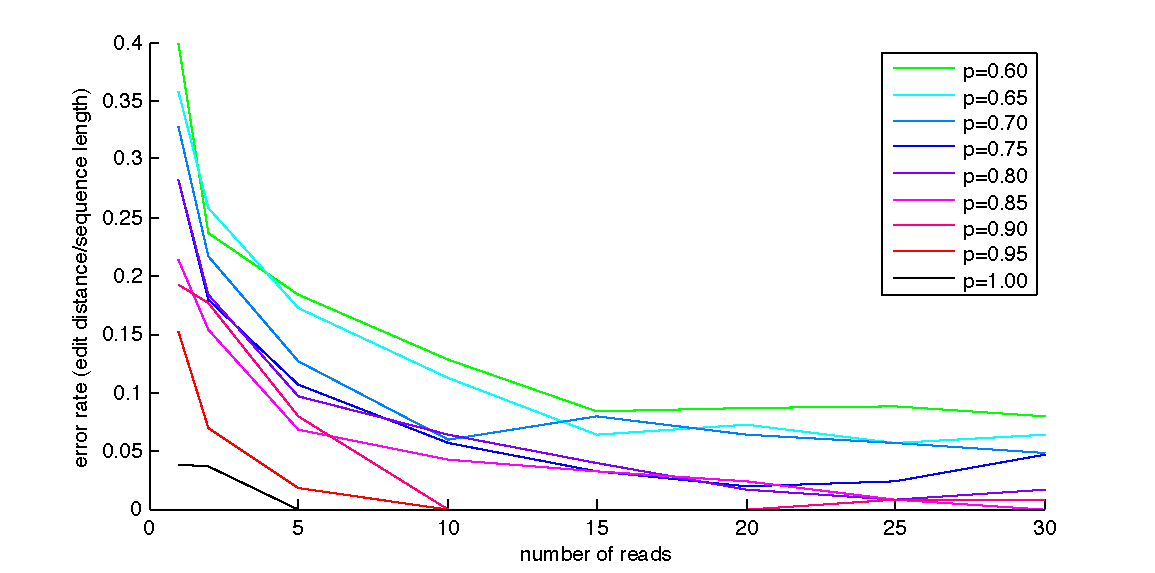
\includegraphics[width=1\textwidth]{fig/np_sweep_n.pdf}
\caption{Inference accuracy as a function of number of reads. Fixed: $e=0.05$, $L=100$. Data is an average of 5 separate trials.}
\label{fig:np_sweep_n}
\end{figure}

\begin{figure}
\centering
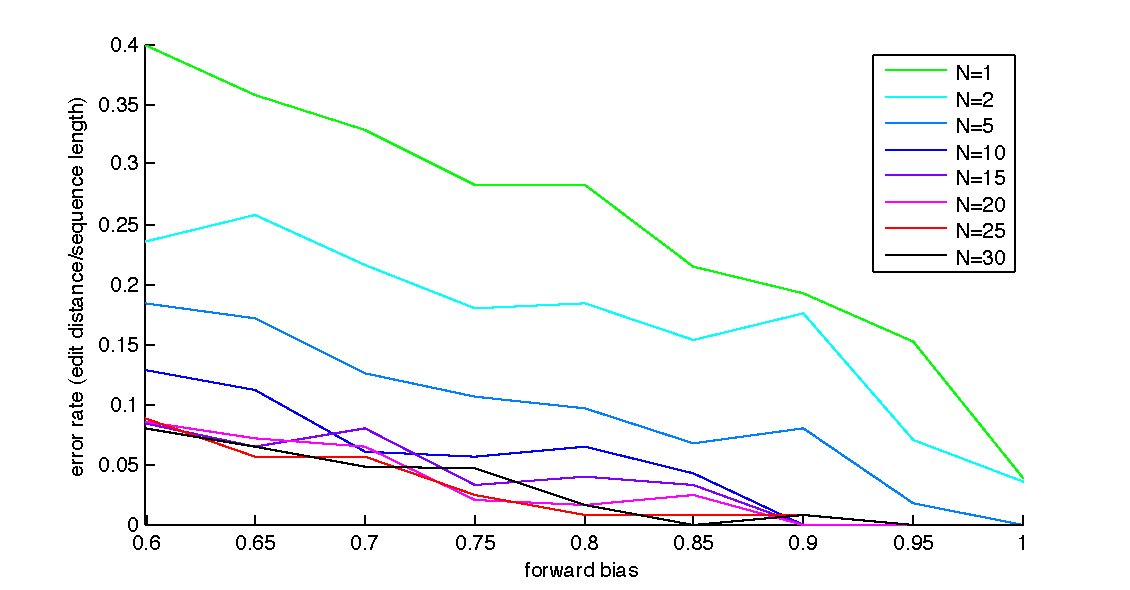
\includegraphics[width=1\textwidth]{fig/np_sweep_p.pdf}
\caption{Inference accuracy as a function of forward bias. Fixed: $e=0.05$, $L=100$. Data is an average of 5 separate trials.}
\label{fig:np_sweep_p}
\end{figure}

Next, we looked at how inference accuracy varies with number of sequence reads for a range of different error values, holding the forward bias fixed at $p=0.75$. Results are plotting in Figure \ref{fig:ne_sweep_e}.

\begin{figure}
\centering
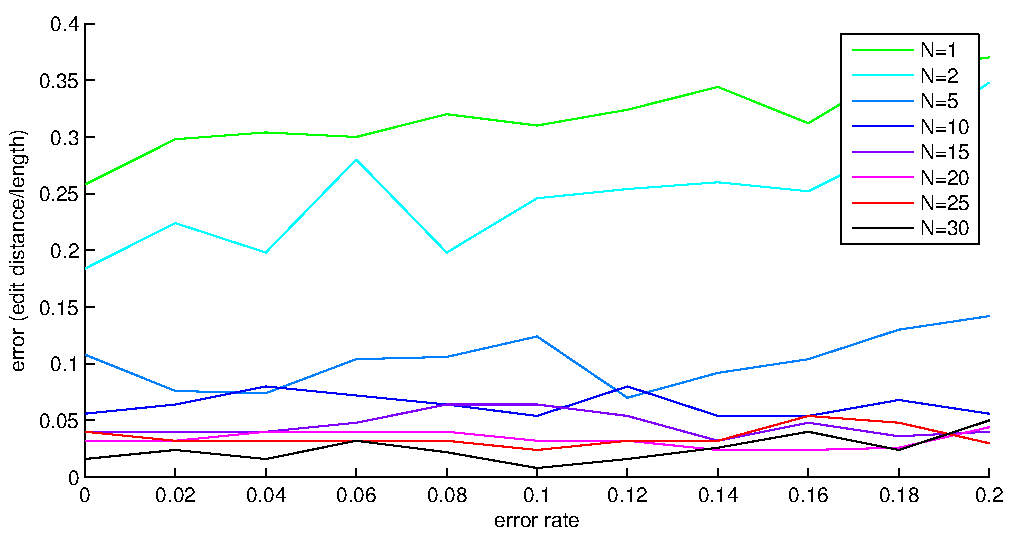
\includegraphics[width=1\textwidth]{fig/ne_sweep_e.pdf}
\caption{Inference accuracy as a function of number of error rate for 8 different number of reads. Fixed: $p=0.75$, $L=100$.}
\label{fig:ne_sweep_e}
\end{figure}

\begin{figure}
\centering
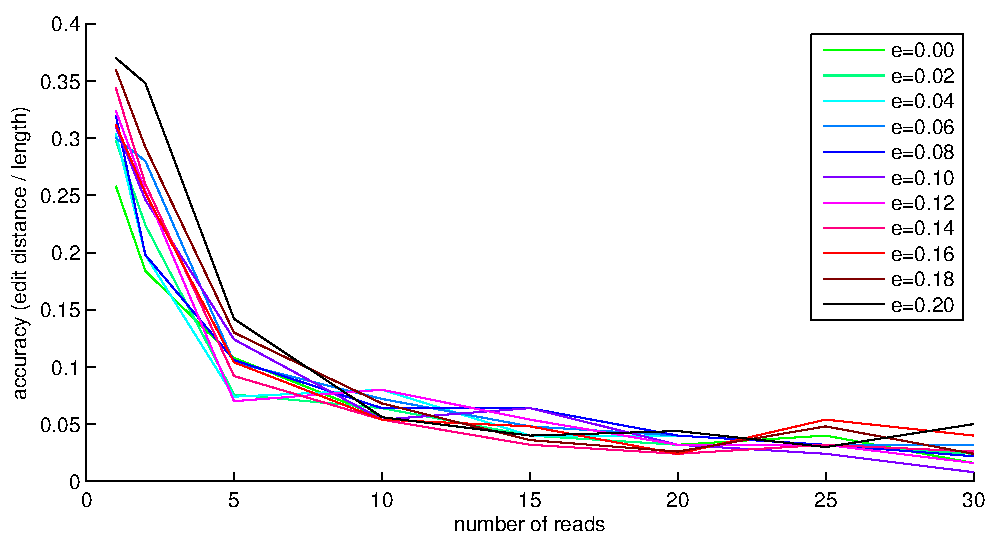
\includegraphics[width=1\textwidth]{fig/ne_sweep_n.pdf}
\caption{Inference accuracy as a function of number of reads for 4 different error rates. Fixed: $p=0.75$, $L=100$.}
\label{fig:ne_sweep_n}
\end{figure}

Finally, Figure \ref{fig:example_inference} shows an example of the algorithm output for the parameter settings $L=100$, $p=0.80$, $e=0.05$, and $N=5$. On the top is plotted the sequence inference as a $4\times L$ colormap, with the true DNA sequence overlaid on top. On the bottom is plotted the information entropy of the sequence inference at each sequence position, where entropy is defined in the usual way as

\begin{equation}
H_l = -\displaystyle\sum_{d}p(S_l=d)\log p(S_l=d).
\end{equation}

This is a typical result in this parameter regime, and is worthy of closer consideration. The edit distance for this example is 4, and examination of the figure quickly shows where the sequence inference deviates from the true sequence. Around position 8 the algorithm misses the CAC pattern, thinking the sequences have in fact moved backwards, and hence is now two steps ahead of the true sequence. The inference is now shifted two postions until reaching position 32, at which point it misinterprets a GAG pattern and returns to the correct sequence. This example demonstrates the general character of the mistakes the algorithm makes -- mistakes generally occur in regions of an ABA pattern, where the algorithm is unable to determine whether the sequences had moved forward or backward. What is notable is that the regions where these shifts occur are also regions of high entropy in the inference, indicating that the algorithm in fact knows that these are troublesome regions. It is likely that a more sophisticated algorithm could be developed that will identify these high entropy areas and perform more robust inference to move out of probable local minima. Altenativelly, more parallel reads can be used to reduce the probability of falling into local minimum corresponding to such a shift. 

\begin{figure}
\centering
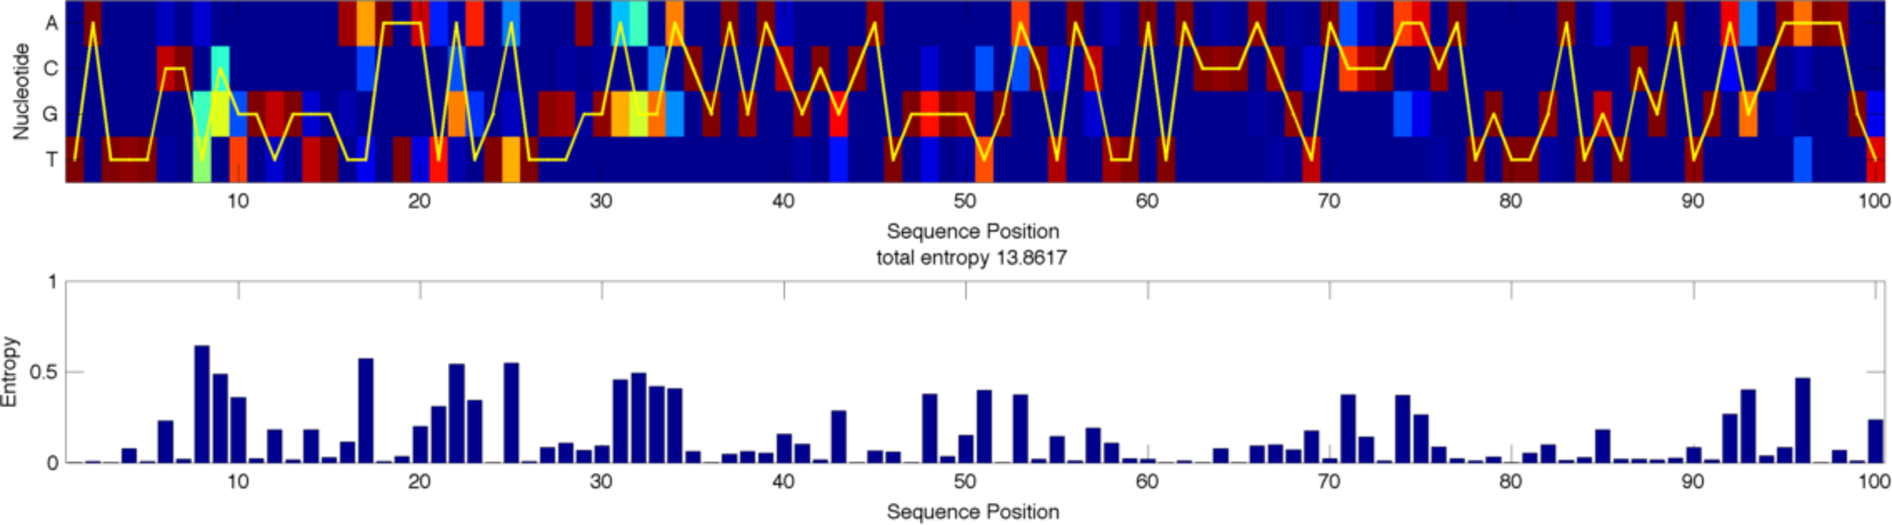
\includegraphics[width=1\textwidth]{fig/example_inference.pdf}
\caption{Top: Inferred sequence distribution. Overlaid is the true DNA sequence. Bottom: Inference entropy at each position. Parameters: $L=100$, $p=0.80$, $e=0.05$, $N=5$.}
\label{fig:example_inference}
\end{figure}

%%\subsection{Scaling}
%%The algorithm is extremely well suited to parallelization, as forward-backward iterations over independent read sequences can be performed in parallel. Scaling to longer sequence lengths is presently an issue, as ideally you would be considering input DNA sequences of $L\approx1000$.

%%The necessary coverage (N) scales inversely with both the likelihood of a backwards step and the accuracy of the base calls.

\section{Discussion}
We have demonstrated that, under the model of DNA translocation as a biased random walk, efficient sequence inference is achievable by combining the results of multiple parallel reads.

In theory, backward steps could be treated as simple insertion errors, but it is important to realize that these insertions are not random but highly correlated with the surrounding sequence. A random walk model allows us to extract useful information from these inserted bases, rather than discarding them as extraneous. As long as the proper walk path is identified, even backward steps effectively serve to increase the read coverage.

Finding the proper walk path, however, is not trivial. The number of possible walk paths for a read sequence of length R is $2^R$, although if p>0.5 then not all paths are equally likely. When base call errors coincide with bidirectional motion the problem becomes particularly difficult. In the limit of p~1, a much simpler version of the presented approach may be implemented, in which one assumes that no more than one or two backwards steps will occur sequentially. This drastically reduces the number of possible walk paths, making it more computationally feasible for very long read lengths.

Designers of nanopore sequencers may find that there is a tradeoff between sequencing speed and maintaining unidirectional motion of the molecules. In this scenario, techniques such as the random walk model may allow throughput to be increased without a loss of accuracy.




%%Additionally, the regular nature of shift errors in the inference suggests that it may be possible to build heuristics to identify these shifts during the inference process, likely by looking at the inference entropy at specific regions. Furthermore, it should be possible to identify areas prone to Future work will proceed in two directions: (1) application of sampling techniques to avoid local minima, and (2) development of techniques to iterateively proceed forward through the sequences in a single pass, rather than multiple forward-backward steps.

% papers to cite:
% branton 2008 - promise of nanopore sequencing
% ibm group in biophysical journal - velocity fluctuations
% samir iqbar book on nanopores
% some experimental papers

\bibliographystyle{plain}
\bibliography{inc/library}

\end{document}
